\documentclass[aps,prl,twocolumn,amsmath,amssymb,superscriptaddress,
longbibliography,floatfix]{revtex4-2}

\usepackage{bm}
\usepackage{graphicx}
\usepackage{xcolor}
\usepackage[colorlinks=true,citecolor=blue!55!black,
urlcolor=blue!55!black,linkcolor=blue!55!black]{hyperref}
\graphicspath{{figs/}}
\setlength{\emergencystretch}{3em}

\newcommand{\bq}{\bm q}
\newcommand{\Szz}{S^{zz}}

% supplemental numbering
\renewcommand{\thesection}{S\Roman{section}}
\renewcommand{\thefigure}{S\arabic{figure}}
\renewcommand{\thetable}{S\arabic{table}}
\renewcommand{\theequation}{S\arabic{equation}}

\begin{document}

\title{Supplemental Material for\\
``Roton-like Reconstruction of the Emergent Photon in Quantum Spin Ice''}

\author{Zhengbang Zhou}
\affiliation{Department of Physics, University of Toronto, Toronto,
Ontario M5S 1A7, Canada}
\author{Yong Baek Kim}
\affiliation{Department of Physics, University of Toronto, Toronto,
Ontario M5S 1A7, Canada}

\date{\today}
\maketitle

Equation numbers of the form (1), (2), \dots\ refer to the main text;
equations of this document are numbered (S1), (S2), \dots

\section{The computed observable and the neutron cross section}
\label{sm:observable}


Throughout, the quantity we compute is the zero-temperature,
sublattice-summed longitudinal correlation function of the local Ising
pseudospin,
\begin{equation}
 \Szz(\bq,\omega)=\frac{1}{N}\sum_{\mu}
 \sum_{n}\big|\langle n|S^z_\mu(\bq)|0\rangle\big|^{2}\,
 \delta\!\left(\omega-\omega_{n}\right),
 \label{eq:szz}
\end{equation}
with
$S^z_\mu(\bq)=\sum_{i\in\mu}e^{-i\bq\cdot\bm r_i}S^z_i$ and $\mu$
running over the four pyrochlore sublattices. Here $S^z_i$ is the
component along the local $\langle111\rangle$ easy axis at site $i$,
which is the component that equals the emergent electric field,
$E_i=S^z_i$. All intensities quoted below --- ``share of the
intensity,'' ``off-pole weight'' --- are fractions of
$\sum_n\sum_\mu|\langle n|S^z_\mu(\bq)|0\rangle|^{2}$ at the same
$\bq$, so they are normalized within Eq.~(\ref{eq:szz}) itself.

Equation~(\ref{eq:szz}) is not the neutron cross-section. The
magnetic neutron cross-section of a non-Kramers or dipolar--octupolar
spin ice involves, in addition, the ionic form factor, the $g$-tensor
projecting the local pseudospin onto the laboratory magnetic dipole,
the rotation from the four local $\langle111\rangle$ frames to the
global frame, and the neutron polarization factor
$\delta_{\alpha\beta}-\hat q_\alpha\hat q_\beta$. Those factors
multiply Eq.~(\ref{eq:szz}) with sublattice-dependent and
$\bq$-dependent coefficients and are material specific; for the
dipolar case they are given explicitly in
Refs.~\cite{Fennell2009,Benton2012}. We do not apply them, because
every statement we make is a comparison between eigenstates \emph{at
the same $\bq$ and in the same sublattice channel}, where these
prefactors are common and cancel from the ratios. They do not cancel
from a comparison between different $\bq$, and we therefore make no
claim about the absolute momentum dependence of neutron intensity.
When we write that a level ``carries half the intensity'' we mean half
of the longitudinal pseudospin weight of Eq.~(\ref{eq:szz}) at that
momentum. Converting to a measured cross-section for a specific
material requires the material's $g$-tensor and is outside the scope
of the pure ring model.

Our calculation is exact within the specified finite Hilbert spaces,
not within the full microscopic spin model. Equation~(1) of the main text
conserves winding, and we work in the ground-state winding sector of
the spin-ice manifold. Electric charges (spinons) are absent by
construction. The magnetic sector is retained, so spectral weight
outside the photon branches could in principle have magnetic rather
than multiphoton character; we distinguish these possibilities below.
A word on which plaquettes enter Eq.~(1) of the main text. A periodic
cluster contains six-site closed loops of two kinds: the elementary
hexagons of the infinite pyrochlore lattice, and loops that close only
by winding around the torus. The latter are not plaquettes of the
lattice, and including them adds ring terms with no counterpart in the
thermodynamic limit; on small clusters they are the majority of all
six-cycles found by a naive search. We therefore keep only loops of
zero winding number, of which the 48-site cluster has exactly $48$,
twelve in each of the four $\langle111\rangle$ orientations. This is
a property of the cluster geometry and is checked directly on each
cluster used here; no result below depends on it being taken on faith.


\section{Cluster construction, sectors, and numerical methods}
\label{sm:methods}

Ice configurations are enumerated exactly by depth-first assignment,
one site at a time, backtracking as soon as any tetrahedron would
acquire a third spin of either sign, and are stored as bit masks. The
ring Hamiltonian is built sparsely: for each hexagon a bit mask and the
two flippable bit patterns identify the acted-on states in one
vectorized pass, and the images are located by binary search in the
sorted state list. The winding sector is identified from the
polarization $\sum_i(n_i-\tfrac12)\bm r_i$, which is conserved by
Eq.~(1) of the main text; we retain the sector carrying the ground state.

On the 48-site cluster the ground-state winding sector has dimension
$9104$ and is diagonalized completely with a dense symmetric
eigensolver, so all $9104$ eigenpairs are available and the
operator-resolved weights saturate the equal-time sum rule
$\sum_n|\langle n|S^z_\mu(\bq)|0\rangle|^2=S_\mu(\bq)$ exactly rather
than to a tolerance. On the 64-site cluster the sector has dimension
$249\,180$ and is treated by Lanczos with full reorthogonalization,
the dynamical response being obtained by a continued-fraction
expansion seeded with $S^z_\mu(\bq)|0\rangle$; all 48-site benchmarks
are reproduced before any 64-site number is quoted.

Going beyond $64$ spins requires changing the state representation.
Storing a configuration in a single $64$-bit word caps the calculation
at $64$ sites, which is where the published constrained-space
spectroscopy has stood. We therefore store each configuration as a
\emph{pair} of $64$-bit words and redefine masking, flipping, sorting
and lookup on that pair. Lookup is the only part that is not
immediate: the table is sorted by the pair lexicographically, and
because the high word takes fewer than $2^8$ distinct values at these
sizes, queries are grouped by high word and each group resolved with a
single vectorized binary search on the low word within its block. The
result is exact, not hashed. The implementation is validated by
running it on the 48-site cluster, where it reproduces the 64-bit
pipeline exactly: $E_0=-10.55601176K$, $S(L)=0.37036$ and branch
energies $1.0235K$ and $1.7303K$.

On the 72-site cluster the ice manifold contains $12\,846\,186$
configurations in $310$ winding sectors. The ground state does
\emph{not} lie in a zero-polarization sector: on this box the
zero-polarization sector is empty, and the two ground sectors are a
degenerate $\pm P$ pair of nonzero integer polarization, each of
dimension $973\,008$. (An earlier version of our tooling labeled the
minimum-$|P|$ sector ``zero-polarization''; we flag this because the
distinction matters for the Monte Carlo initialization of
Appendix~\ref{sm:gfmc}, which must reach this nonzero-$P$ sector.)
The identification is verified rather than assumed, by diagonalizing
the largest sectors independently and comparing, which also exposes
the expected exact degeneracy between the $\pm P$ pair, both at $E_0=-14.80971536K$. The dynamical response is again
obtained by continued fraction seeded with the four sublattice
components of the probe. Because those four seeds produce separate
lines at the same energy, they are summed by energy before any branch
energy or weight is quoted; only the channel sum is
basis-independent.

The 96-site cluster required two further steps. The two-billion-state
ice manifold is enumerated by a vectorized frontier that imposes one
tetrahedron at a time, visiting at each step the tetrahedron that
introduces the fewest new sites and branching the frontier into
independent seeds so that peak memory is bounded by one branch
(a hundredth of a gigabyte) rather than the whole frontier; and exact
state lookup is a single lexicographic \texttt{searchsorted} on the
$(\mathrm{hi},\mathrm{lo})$ word pairs, since at this size a
block-by-block search over the $\sim$millions of distinct high words
is no longer viable. The winding sector is identified from an exact
integer polarization key without sorting the manifold, candidates
estimated from a four-million-state sample and each extracted in one
masked pass; the ground sector (dimension $146\,758\,352$, $2.7\times
10^{9}$ nonzeros) is identified by diagonalizing the largest
candidates and comparing. What excludes a smaller sector from lying
lower: at 48 and 72 sites, where every winding sector can be
enumerated and the largest ones diagonalized, the ground state always
lies in a sector of maximal dimension, with sub-leading sectors
higher by $O(1)K$; at 96 sites we verify this for the three largest
candidates directly and rely on the same pattern for the rest. On the
cubic Monte Carlo boxes the sector reached by the seed randomization
is certified by the energy gate of Appendix~\ref{sm:gfmc}, which
resolves a wrong sector at the percent level in $E_0/N$ against a
statistical error two orders smaller. The continued fraction uses real Lanczos on
the real and imaginary parts of each probe separately, which is exact
for a real symmetric $H$ and halves the Krylov storage; $120$
iterations reproduce the $250$-iteration complex results on the
72-site cluster to every digit.

Momentum labels are certified by explicit translation projectors

\subsection{Sector certification}
\label{sm:sectors}

% SECTCERT-PLACEHOLDER: exhaustive 48/72 + top-12 at 96 (job 19461223)

\subsection{Krylov convergence at 96 sites}
\label{sm:krylov}

% KRYLOV-PLACEHOLDER: omega(m), Z(m), residuals from the stored
% tridiagonals + the 120-vs-200 iteration comparison (job 19440533)

\section{The Gaussian benchmark}
\label{sm:gaussian}


Every statement of the form ``about half the Gaussian-photon energy''
refers to the following construction, which is quantized on the same
finite torus as the exact diagonalization so that no continuum
extrapolation enters the comparison.

Write $B_p=\sum_\ell C_{p\ell}A_\ell$, where $C$ is the alternating
lattice curl: $C_{p\ell}=\pm1$ with alternating sign around the six
links of hexagon $p$, and zero otherwise. Expanding the compact
magnetic energy of Eq.~(1) of the main text to quadratic order and adding
the electric term gives
\begin{equation}
 H_G=\frac{U}{2}\sum_\ell E_\ell^2+K\sum_p B_p^2 ,
 \qquad [A_\ell,E_{\ell'}]=i\delta_{\ell\ell'} .
 \label{eq:hg}
\end{equation}
Restricting to momentum $\bq$ and using the four-dimensional
sublattice Bloch basis, the normal-mode frequencies are set by the
singular values $\sigma_\lambda(\bq)$ of the curl in that block,
\begin{equation}
 \omega_\lambda(\bq)=\sqrt{2UK}\;\sigma_\lambda(\bq) .
 \label{eq:gaussdisp}
\end{equation}

The construction is checked, not assumed. (i)~Gauge invariance:
$C\,d_0=0$ to machine precision, where $d_0$ is the tetrahedron
incidence matrix signed by the up/down bipartition; the largest
element of $Cd_0$ is $0$ exactly. If this fails the sign convention
is wrong and nothing downstream is meaningful. (ii)~At every
$\bq\neq\Gamma$ the block has exactly two nonzero singular values, the
two transverse photon polarizations, and at $\Gamma$ it has none.
(iii)~The Bloch bases are orthonormal, and the probe at $+\bq$ pairs
with modes at $-\bq$, verified by projection completeness.

A single number is fitted: the overall energy scale $\sqrt{2UK}$. In
the pure ring model $U$ is generated dynamically rather than being a
bare coupling, so its value is not available from Eq.~(1) of the main text;
this is the one place where we import a scale from the data. It is
determined by one linear least-squares fit of the dominant exact line
against the dominant Gaussian branch across all momenta, giving
$\sqrt{2UK}=0.5868\,K$. Everything else --- the \emph{shape} of the
dispersion across momenta, the degeneracy or splitting of the two
polarizations at each $\bq$, and the distribution of one-photon weight
over momenta and sublattice channels --- is parameter-free geometry.
The resulting values are those plotted as the dashed Gaussian curve
of Fig.~1 of the main text; at $L$, $\omega_{\rm G}=2.03K$.

We stress the limitation this creates. Because one scale is fitted to
the exact spectrum, the Gaussian curve cannot be used to test whether
the overall photon velocity is renormalized: by construction it is
not. It can only be used for statements that are invariant under a
uniform rescaling of the whole branch --- which momenta are anomalous
\emph{relative to the others}, and whether the two polarizations split.
Those are the only statements we draw from it.


\section{Basis-invariant polarization resolution}
\label{sm:polar}


At each momentum the electric field lives in the four-dimensional
sublattice space, in which the lattice curl has exactly two nonzero
singular values. The neutron probe is therefore confined to a
two-dimensional transverse subspace; the weight found in the remaining
two directions is the longitudinal residue, which must vanish because
$\nabla\!\cdot\!\bm E=0$ in the ice manifold. It does, at the level of
$10^{-31}$ relative to $S(\bq)$ at every momentum. This is an exact
gate on the decomposition, not a fit.

A caution is necessary before any polarization statement is made. The
two Gaussian transverse branches are \emph{exactly} degenerate at every
momentum, so the singular-value decomposition determines the two
polarization directions only up to an arbitrary rotation within that
subspace. A statement such as ``this level is $68\%$ polarization~1''
is consequently meaningless in isolation. The invariant content is
the geometry of the levels' polarization vectors relative to one
another. For a level $n$ of multiplicity $m$ we form the $2\times2$
polarization density matrix $M_n=A_n^\dagger A_n$, where $A_n$ is the
$m\times2$ matrix of transverse amplitudes
$\langle n,\alpha|S^z(\bq)|0\rangle$. Both the purity
$\mathrm{tr}\,M_n^2/(\mathrm{tr}\,M_n)^2$ and the normalized overlap
$\mathrm{tr}(M_AM_B)/(\mathrm{tr}\,M_A\,\mathrm{tr}\,M_B)$ between two
levels are invariant under rotations of the degenerate subspace.

The result is unambiguous. Every bright level, including multiplets
of multiplicity up to four, has polarization purity $1.000000$: the
whole multiplet couples through a single polarization direction. And
the two brightest levels at each momentum are mutually orthogonal in
polarization, so a basis exists in which each is pure. They are
therefore the two transverse photon descendants, identified without
reference to any energy scale.

\begin{center}
\begin{tabular}{lrrrr}
\hline\hline
$\bq$ & $\omega_1/K$ & $\omega_2/K$ & splitting & overlap\\
\hline
$(\frac13,\frac13,\frac13)$ & $1.895$ & $1.980$ & $0.044$ & $2\times10^{-28}$\\
$(\frac13,\frac13,\frac23)$ & $1.744$ & $2.069$ & $0.171$ & $1\times10^{-29}$\\
$(\frac16,\frac16,\frac56)$ & $2.533$ & $2.687$ & $0.059$ & $4\times10^{-2}$\\
$L$                         & $1.024$ & $1.730$ & $0.513$ & $3\times10^{-3}$\\
$X$                         & $2.235$ & $3.423$ & $0.420$ & $1\times10^{-31}$\\
\hline\hline
\end{tabular}
\end{center}

The splitting column is
$|\omega_1-\omega_2|/\tfrac12(\omega_1+\omega_2)$, the convention used
throughout this paper; normalizing instead by the lower branch would
give larger numbers for the same data. Orthogonality is
exact to machine precision at $(\frac13,\frac13,\frac13)$,
$(\frac13,\frac13,\frac23)$ and $X$, where the little group forbids
mixing, and holds to $0.3\%$ at $L$ and $4\%$ at
$(\frac16,\frac16,\frac56)$, where it does not. The residual mixing
is small enough that the branch assignment is never in doubt.

Two consequences matter for the interpretation. First, the
identification of the anomalous $L$ level as a photon descendant, and
not a new species, rests on this decomposition and is independent of
the fitted Gaussian scale. Second --- and this must be stated
plainly --- the ``interaction-induced polarization splitting'' and the
``roton-like softening'' at $L$ are not two independent findings.
They are the same fact viewed twice: the lower of the two transverse
branches at $L$ is the anomalous level, and the splitting between the
branches is the amount by which it has been pushed down. We report
the splitting because it connects to a specific earlier
prediction~\cite{Kwasigroch2017,Kwasigroch2020}, not as separate
evidence.


\section{The Rokhsar--Kivelson deformation and the census}
\label{sm:census}

classify the eigenstates we use the conventional Rokhsar--Kivelson
extension of the pyrochlore ring model,
\begin{equation}
 H(V)=-K\sum_p\!\left(W_p+W_p^\dagger\right)
      +V\sum_p n_p^{\rm flip},
 \label{eq:rk}
\end{equation}
where $n_p^{\rm flip}$ projects onto an alternating hexagon, so that
$\sum_p n_p^{\rm flip}$ simply counts the flippable plaquettes in a
configuration. The sign convention matters for reading the figures
and we state it once: $V>0$ penalizes flippable plaquettes, $V<0$
rewards them, and the exactly solvable Rokhsar--Kivelson point sits at
$V=+K$, where the equal-amplitude superposition is an exact ground
state. Our scans run over $V/K\in[-0.5,+0.5]$ unless stated
otherwise, and the anomalous level softens toward negative $V$, that
is, toward configurations with more flippable plaquettes. This
flippability potential was introduced for the pyrochlore ring model in
the original gauge-theory construction and subsequently used to map
the quantum-ice phase diagram and tune the emergent electrodynamics
~\cite{Hermele2004,RokhsarKivelson1988,Shannon2012,Pace2021}. Our use
of it is different. We remain at the physical ring point $V=0$ and
use only the infinitesimal derivative of an individual excitation
energy. Hellmann--Feynman gives
\begin{equation}
 \frac{d\omega_n}{dV}
 =\langle n|\!\sum_p n_p^{\rm flip}|n\rangle
 -\langle 0|\!\sum_p n_p^{\rm flip}|0\rangle ,
 \label{eq:hf}
\end{equation}
so the slope is an exact state-resolved census of the number of
flippable hexagons added or removed by the excitation. No parameter is
fit to obtain this diagnostic.

At $L$ the two strongest $S^z$-active levels respond with opposite
signs. The level at $1.73K$, close to the Gaussian-photon energy
$2.03K$, loses flippable hexagons as $V$ is increased and behaves as an
ordinary dressed photon. The lower level at $1.02K$ carries $51\%$ of
the $S^z$ spectral weight and gains flippable hexagons. It is also the
lowest eigenvalue in the fully diagonalized 9104-dimensional
48-site ground-state winding sector, including both spin-reversal
parities. We do not elevate that finite-sector statement to a claim
about all winding sectors or about the full microscopic spin model.
Parity excludes only even photon number; the three-photon channel is
excluded separately, and by a wide margin, on kinematic grounds
(Sec.~\ref{sm:kin}), while the flux-correlation diagnostic
discussed below disfavors a localized magnetic pair. The combination
of collective ancestry, strong finite-momentum softening, and
qualitatively different microscopic response motivates the roton-like
terminology.

\label{sec:census-limits}

It is tempting to read the census as a sign rule: an excitation
disrupts ring resonance, so it should \emph{lose} flippable plaquettes,
and a level that gains them is thereby marked as different in kind.
That reading is too strong, and the exact statement is worth having
because it says precisely how much is true.

The operator $N=\sum_p n_p^{\rm flip}$ is diagonal in the
configuration basis, and each flippable hexagon of a configuration
contributes exactly one off-diagonal element of the ring Hamiltonian.
Hence $\mathrm{Tr}\,N$ equals the number of nonzero off-diagonal
elements of $H$, and the census averaged over \emph{all} eigenstates of
a sector of dimension $D$ is
\begin{equation}
 \frac{1}{D}\sum_{n}\frac{d\omega_n}{dV}
 =\frac{\mathrm{nnz}(H)}{D}-\langle 0|N|0\rangle ,
 \label{eq:censussum}
\end{equation}
which is negative precisely because the ground state is more flippable
than a typical ice configuration. On the 48-site cluster
Eq.~(\ref{eq:censussum}) gives $-0.9139$, and direct diagonalization of
all $9104$ eigenstates returns the same number to $10^{-14}$.

So excitations do lose flippability on average, exactly and provably.
Nothing, however, constrains an individual level. Of the $9104$
eigenstates, $58$ --- $0.64\%$ --- have a positive census, and $20$
exceed $+0.20$. The anomalous $L$ level at $+0.339$ sits in that top
$0.22\%$ tail, which is the honest form of the statement: it is
extreme, not unique.

The census is also the least size-stable of our diagnostics, and we say
so plainly. At the anomalous level it is $+0.339$ on 48 sites,
$+0.338$ on 64, $+0.134$ on 72 and $+0.259$ on 96. The sign is
robust; the magnitude is not, and no normalization we tried repairs
it. On 48 and 64 sites the anomalous level is the only appreciably
positive bright census, exceeding the next by factors of $29$ and $7$;
on 72 sites several bright levels are positive and it is no longer the
largest. We therefore do not use the census as the primary
discriminant.

What does survive on every cluster is a comparison made \emph{within}
one of them, and it now appears at two sizes. The 64- and 96-site
boxes each carry two inequivalent $L$-type classes
at identical $|\bq|$ and identical Gaussian energy. The class that
reconstructs has census $+0.338$ (64) and $+0.259$ (96); the class
that does not has
$-0.166$ and $-0.02$/$-0.09$ respectively. Same momentum star, same
free-theory prediction, opposite
response to the flippability probe. That contrast needs no comparison
across cluster sizes and no fitted scale, and it is the census evidence
we rely on.

\section{Why the ratio is small near $L$: geometry, amplitudes, and controls}
\label{sm:whyL}

Two ingredients coincide at
this momentum. The first is geometric. A hexagon contained in a
wavefront, i.e. in a plane of constant phase perpendicular to $\bq$,
encloses zero flux from the electric-field wave: the alternating loop
sum defining $g_p$ vanishes exactly. Such a plaquette contributes
nothing to the first-moment expression $f_1$ [Eq.~(9) of the main text]. Pyrochlore hexagons are perpendicular
to the four $\langle111\rangle$ directions, and at the sampled
zone-boundary point $L\parallel[111]$ one of the four hexagon families
lies in the wavefronts. That family therefore drops out of the
oscillator-strength cost exactly, and the vanishing is an identity, not
a small number: resolved by family, the geometric factor
$\sum_p\sum_\mu|g^\mu_p(\bq)|^2$ at $L$ is $(96,96,96,0)$, against
$(96,96,96,96)$ at $X$. The reduction of the \emph{geometric} factor
is therefore exactly $3/4$. The reduction of $f_1$ itself is not
exactly $3/4$, because the first-moment expression $f_1$ [Eq.~(9) of the main text] weights each plaquette by its
own ring coherence $w_p=\langle W_p+W_p^\dagger\rangle$, which is not
uniform on an anisotropic cluster; numerically
$f_1(L)/f_1(X)=0.684/0.880=0.777$.

It is important that this geometric decoupling is necessary but not
sufficient. It occurs at every momentum along $[111]$: at the smallest
such momentum the family resolution is $(72,0,72,72)$, again with one
family exactly dark. Yet that momentum shows no anomaly, its dominant
level sitting at $1.98K$ against a Gaussian value of $1.76K$. What
distinguishes $L$ is the second ingredient below.

The second ingredient is dynamical. In the interacting $V=0$ ground
state the equal-time structure factor is largest at $L$ among the
sampled momenta: $S(L)=0.370$, compared with $0.19$--$0.29$ elsewhere.
The combination of reduced $f_1$ and enhanced $S$ makes
$f_1/S$ smallest at $L$ among the twelve cluster momenta and makes it
the only sampled point where the single-mode energy falls below the
Gaussian-photon line.

Crucially, the enhancement of $S(L)$ is not inherited from the ice
constraint alone, and two independent controls establish this.

The first is exact and requires no sampling. The equal-amplitude
superposition over the \emph{same} $9104$ configurations of the
\emph{same} cluster is the classical ice ensemble restricted to
exactly what the quantum state can reach, so comparing it with the
interacting ground state isolates the effect of the amplitudes alone.
It gives $S(L)=0.297$ against the interacting value $0.370$. Measured
as an enhancement over the other sampled momenta, the classical
ensemble raises $L$ by $11\%$ and the interacting ground state by
$48\%$. Roughly four fifths of the $L$ enhancement is therefore made
by the quantum dynamics, not by the ice rule.

The second checks that this is not an artifact of the small cluster.
Loop-update Monte Carlo on a 2048-site classical ice manifold, binned
into $30$ independent blocks, gives
$S(L)=0.2488(67)$, $S(X)=0.2538(73)$, $S(W)=0.2475(52)$ and
$S(K)=0.2467(46)$. The total spread across these zone-boundary
momenta, $0.007$, is comparable to the typical statistical error,
$0.006$: within the resolution of the calculation the classical
structure factor is flat, and $L$ in particular is not distinguished.
(The zone center is excluded from this comparison; it is the uniform
mode, and it carries no weight in the finite cluster.) The much
stronger $L$ enhancement seen in the interacting ground state is
generated by the quantum ring dynamics at $V=0$. This is the main
distinction from an RK-point resonon, whose softening can be read
directly from the classical correlations of the equal-amplitude state.

Finally, the mechanism is the \emph{ratio}, and $L$ is where the ratio
is minimized rather than a privileged point in itself. The 72-site
cluster makes this concrete: its momentum $(\frac16,\frac12,\frac12)$
has a family decomposition $(36,144,144,108)$ --- one hexagon family
suppressed to a quarter rather than the exact zero that $L$ enjoys ---
but a structure factor almost as large, and its ratio comes out within
$0.9\%$ of the $L$ value. Its spectrum is correspondingly almost
identical: a dominant level at $1.075K$ with $55\%$ of the weight,
against $1.068K$ with $54\%$ at $L$. Exact geometric decoupling is
therefore one route to a small ratio; partial suppression combined
with a large $S(\bq)$ is another, and the spectrum follows the ratio,
not the route.


\section{Finite-size and deformation checks}
\label{sm:finite}


\begin{figure}[t]
\centering

\includegraphics[width=\columnwidth]{fig_dssf.pdf}
\caption{The mode itself: exact $\Szz(\bq,\omega)$ near $L$. (a) The
 72-site spectrum at five momenta, each normalized by its own
 $S(\bq)$; the poles are Lanczos-converged (sum-rule gate $1.0000$),
 broadened by a display-only
 $\eta=0.05K$. At the three photon-like momenta the response peaks at
 $1.5$--$2.2K$; at $L$ \emph{and} at the soft-valley momentum
 $(\frac16,\frac12,\frac12)$ (Sec.~\ref{sm:valley}) it collapses
 onto a single dominant pole near $1K$ carrying over half the weight
 (shaded band). (b) The $L$-point spectrum at all four diagonalized
 sizes, overlaid: the soft pole sits at $0.90$--$1.07K$ with about
 half the weight at every size, the upper transverse branch at
 $1.65$--$1.81K$. Nothing here is fitted or extrapolated; the figure
 is the spectrum.}
\label{fig:dssf}
\end{figure}
\emph{Convergence of the collective state.} A systematic variational
improvement of the electric-field wave converges rapidly to the exact
48-site eigenvalue, $1.450\to1.074\to1.034\to1.026K$ against $1.024K$
from complete diagonalization. The state is reached from the probe in
a few steps, as a collective mode should be, rather than requiring the
full Hilbert space.

\emph{A prediction, not a fit.} The 64-site cluster provides the one
test in which the ground-state ratio is used in the direction it is
supposed to work: forward. Its anisotropy splits the $L$ star into two
inequivalent classes, which the Gaussian theory cannot distinguish ---
both have the same $|\bq|$ and the same Gaussian energy. They differ
in a ground-state quantity, the equal-time structure factor:
$S=0.369$ for one class and $S=0.227$ for the other. The $f_1/S$
mechanism therefore predicts, before any excited state is computed,
that the first class reconstructs and the second does not. It does.
The class with $S=0.369$ carries a level at $0.954K$ with $50.0\%$ of
the weight; the class with $S=0.227$ has its dominant level at
$1.998K$ with $77\%$ of the weight, and no anomalous state at all.
The effect follows the structure factor rather than the label $L$.

\emph{Stability with size.} We can now compare four clusters. The
third, $2{\times}3{\times}3$ with 72 spins, required extending the
state representation past a single 64-bit word; the fourth,
$2{\times}3{\times}4$ with 96 spins, required in addition a vectorized
enumeration of its two-billion-configuration ice manifold and a
Lanczos treatment of a $146\,758\,352$-dimensional winding sector
(Appendix~\ref{sm:methods}). Ninety-six spins matches the largest
constrained-space exact diagonalization reported for this model
~\cite{Pace2021}, there used for ground-state properties; here the
full operator-resolved response is obtained. The four boxes span
three distinct shapes.

\begin{center}
\begin{tabular}{lrrrr}
\hline\hline
 & $2{\times}2{\times}3$ & $2{\times}2{\times}4$ &
   $2{\times}3{\times}3$ & $2{\times}3{\times}4$\\
sites & $48$ & $64$ & $72$ & $96$\\
ice configurations & $87\,546$ & $2.76{\times}10^{6}$
  & $1.28{\times}10^{7}$ & $2.01{\times}10^{9}$\\
sector dimension & $9\,104$ & $249\,180$ & $973\,008$
  & $1.47{\times}10^{8}$\\
\hline
$E_0/N$ & $-0.2199$ & $-0.2165$ & $-0.2057$ & $-0.2038$\\
$S(L)$ & $0.370$ & $0.369$ & $0.321$ & $0.355$\\
$\omega_{\rm low}/K$ & $1.024$ & $0.954$ & $1.068$ & $0.904$\\
share & $50.8\%$ & $50.0\%$ & $54.0\%$ & $54.4\%$\\
$\omega_{\rm high}/K$ & $1.730$ & $1.652$ & $1.814$ & $1.647$\\
$\omega_{\rm low}/\omega_{\rm high}$ & $0.592$ & $0.578$ & $0.589$
  & $0.549$\\
census $d\omega_{\rm low}/dV$ & $+0.34$ & $+0.34$ & $+0.13$ & $+0.26$\\
\hline\hline
\end{tabular}
\end{center}

The qualitative picture is identical on all four: a single dominant
level near $1K$ carrying at least half of the weight at $L$, and a
second transverse branch roughly seventy percent higher. The
scale-free ratio of the two branch energies varies over
$0.549$--$0.592$ across a factor of $16\,000$ in sector dimension and
three box shapes; the soft level's share of the weight varies over
$50$--$54\%$. This is the evidence least contaminated by fitted
quantities. On the largest cluster the mode is, if anything, the
softest of the four.

\emph{The class prediction repeats at 96 sites.} The
$2{\times}3{\times}4$ box, like the 64-site one, carries two
inequivalent $L$ classes, with $S=0.355$ and $S=0.241$. Computed
before any excited state, the ratio again selects the first: it
develops the $0.904K$ level with $54.4\%$ of the weight, while the
second remains photon-like, its two dominant levels at $1.651K$ and
$1.730K$ with flippability censuses of $-0.02$ and $-0.09$ against
$+0.26$ for the soft mode. The forward discrimination between $L$
classes has therefore succeeded at two sizes independently, and the
census contrast within a single cluster --- positive for the class
that reconstructs, negative at the same $|\bq|$ for the class that
does not --- appears at both.

Not everything is stable, and we say which. $S(L)$ moves between
$0.321$ and $0.370$ with box shape; the weight retained by the upper
branch varies between $18\%$ and $32\%$; the census magnitude varies
by a factor $2.6$ (Sec.~\ref{sec:census-limits}); and the polarization
splitting at $X$ is not converged, falling from $42\%$ at 48 sites to
$5.9\%$ at 64; no conclusion is drawn from it.

\emph{The deformation trajectory.} Under a bias toward more flippable
configurations ($V<0$), $f_1(L)$ changes by less than one percent
while $S(L)$ grows and the level softens from $1.02K$ to $0.73K$. The
ground-state factor moves first and the spectrum follows, which is the
ordering the $f_1/S$ mechanism requires and the opposite of what a
fitted correlation would produce.



\section{The soft valley}
\label{sm:valley}

A quasiparticle minimum should be concave up, and one should ask in
which directions it is, and whether the softness is confined to a
single point. The complete grid answers both. Away from $L$ the ratio
rises in \emph{every} allowed non-radial direction: to $2.216(5)$ at
$(\frac14,\frac12,\frac12)$, to $2.265(5)$ at
$(\frac38,\frac38,\frac58)$, to $2.484(5)$ at
$(\frac14,\frac12,\frac34)$, and steeply to $2.78$ at $W$ --- so $L$
is a genuine minimum of the landscape, not a saddle among the
zone-boundary momenta. (Along the radial $[111]$ line the point is
stationary by band periodicity, as at any zone corner; a lattice
minimum lives in the boundary manifold, exactly as the magnon
roton-like minima of frustrated antiferromagnets do at their zone
corners.)

The rise is, however, strongly anisotropic: the landscape at 2048
sites has a shallow \emph{valley} along the $(t,\frac12,\frac12)$
lines, with the ratio varying by only two percent from
$(0,\frac12,\frac12)$ through $(\frac14,\frac12,\frac12)$ to its
minimum at $L$, while every direction transverse to the valley climbs
by $15$--$28\%$. The softness is therefore not an isolated point: it
is the bottom of a flat trough. And this is not only a statement
about the centroid: the 72-site cluster carries a momentum on exactly
this line, $(\frac16,\frac12,\frac12)$, and its \emph{exact} spectrum
shows a soft level at $1.075K$ with $55\%$ of the weight ---
essentially degenerate with the $L$ mode at $1.068K$
(main text). The prediction that the trough hosts
soft modes away from $L$ is thus verified spectrally at the one
accessible momentum on it. A flat valley of nearly degenerate soft
collective modes, rather than a single deep pocket, is itself a
statement about the physics: whatever ordering tendency the softening
signals is frustrated among the wavevectors of the valley.


\section{Few-photon kinematics}
\label{sm:kin}


Spin-reversal parity alone does not identify the low $L$ level. Under
charge conjugation an $n$-photon state carries parity $(-1)^n$, so the
odd parity of the level excludes even photon number but permits $n=3$.
We therefore test the three-photon assignment kinematically. Using the
Gaussian branch quantized on the same torus
(Appendix~\ref{sm:gaussian}), we minimize the total energy over every
partition of the cluster momentum into $n$ photon momenta drawn from
the allowed set, excluding $\Gamma$, which carries no photon because
the curl has no nonzero singular value there. At $L$ the resulting
thresholds are
\begin{equation}
 \omega^{(1)}_L=2.03K,\qquad
 \omega^{(2)}_L=4.03K,\qquad
 \omega^{(3)}_L=5.55K .
 \label{eq:thresholds}
\end{equation}
The level in question lies at $1.02K$, a factor of $5.4$ below the
three-photon threshold and below even the one-photon energy. The same
ordering holds at every sampled momentum: the three-photon threshold
never falls below $5.28K$, because the softest photon available on this
cluster already costs $1.76K$. A three-photon state built from weakly renormalized Gaussian
photons is therefore excluded on the clusters we can diagonalize;
since the paper itself establishes that interactions at the zone
boundary are order one, this is a statement about that description,
not a kinematic theorem about arbitrarily dressed constituents.

This argument uses the Gaussian dispersion to count the cost of the
constituents, and so it is an argument about weakly renormalized
photons. It does not by itself exclude a multiparticle state built
from strongly renormalized constituents. What makes that alternative
implausible here is that the level is a single, sharp, dominant pole
carrying half of the weight at its momentum rather than the small
distributed weight characteristic of a continuum, and that its
polarization content is that of a single transverse branch
(Appendix~\ref{sm:polar}).


\section{Off-pole weight and the polarization splitting}
\label{sm:offpole}

The two transverse polarizations are exactly degenerate in the
Gaussian theory, and their interaction-induced splitting was predicted
in semiclassical treatments~\cite{Kwasigroch2017,Kwasigroch2020}. Our
calculation determines its magnitude in the microscopic ring model
without an expansion. Because the two brightest levels at each
momentum are polarization-pure and mutually orthogonal
(Appendix~\ref{sm:polar}), the splitting can be read off
directly as the energy difference between them. It grows
monotonically as the momentum increases: it is unresolved, below the
$10^{-8}K$ level-grouping tolerance, at the smallest momentum of the
64-site cluster, $4.4\%$ at the smallest momentum of the 48-site
cluster, $17\%$ at $(\frac13,\frac13,\frac23)$, $42\%$ at $X$ and
$51\%$ at $L$. The degeneracy is thus restored in the infrared, as
the Gaussian theory requires, and destroyed at the zone boundary.

We emphasize what this does \emph{not} add. The splitting at $L$ and
the roton-like softening at $L$ are the same fact: the softened level
is the lower of the two transverse branches, and the splitting is the
size of the softening. It is reported here because it makes contact
with a specific earlier prediction, not as independent evidence for
the anomaly.

Beyond the two photon descendants, $16$--$38\%$ of the $S^z$ spectral
weight resides in higher levels absent from the Gaussian one-photon
theory. This fraction is defined without any energy window or fitted
scale: the two photon descendants are identified as the brightest
level in each transverse polarization channel, and the off-pole weight
is everything else (Appendix~\ref{sm:polar}). An alternative
operational definition --- simply the two brightest levels at that
momentum --- gives identical numbers at every momentum sampled. The
off-pole fraction takes its smallest value, $16\%$ on 48 sites and
$13\%$ on 64 sites, at the smallest momentum available on each,
consistent with recovery of the infrared photon.

Several diagnostics favor a multiparticle rather than a localized
magnetic interpretation of this higher weight. Plaquette-flux
correlations are weak and spatially extended instead of showing the
localized disturbance expected for a bound magnetic pair, and the
response to the RK deformation is consistent with sums of single-mode
responses. By contrast, leading-order perturbation theory in the
quartic term obtained by expanding the cosine predicts polarization
splittings and transferred spectral weight below $0.1\%$ at the
coupling generated by this model, and only a few percent even when that
coupling is artificially tripled. The finite-momentum spectrum is
therefore not quantitatively described as a weak anharmonic correction
to the Gaussian photon.


\section{Parity and complementary probes}
\label{sm:parity}

Global spin reversal leaves
Eq.~(1) of the main text invariant. Eigenstates can therefore be chosen
even or odd under this symmetry, while $S^z$ is odd. Consequently a
spin-reversal-even ground state couples through neutron scattering only
to odd states. This elementary selection rule is exact in the model;
numerically every even level carries $S^z$ weight below $10^{-28}$.
In gauge language it is charge conjugation, under which an $n$-photon
state has parity $(-1)^n$.

The practical implication is a clean division between linear and
bilinear probes. Even-sector weight, including the two-photon channel,
is invisible to $S^z$ but can appear in probes coupling to spin pairs,
such as Raman scattering~\cite{Fu2017} and ultrasound~\cite{Simon2022}.
Stray-field noise magnetometry~\cite{Naik2026}, which couples to
magnetization, belongs to the neutron-like odd channel. The selection
rule itself is not a new symmetry statement; its value here is that the
complete finite-size spectrum makes the complementary experimental
channels explicit.

\begin{figure}[t]
\centering
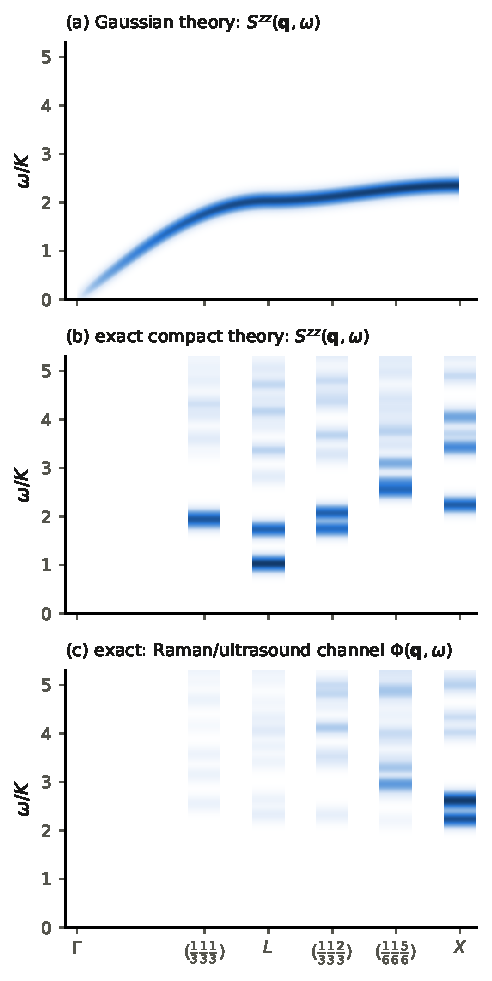
\includegraphics[width=\columnwidth]{fig_maps.pdf}
\caption{Simulated spectra along $\Gamma$--$L$--$X$ for the 48-site
 cluster, broadened by $\eta=0.08K$ and normalized separately in each
 panel. (a) Gaussian one-photon neutron response. (b) Exact
 operator-resolved $S^z$ response within the ground-state winding
 sector: split photon descendants, a dominant low $L$ mode at about
 half the Gaussian-photon energy, and higher off-pole weight. (c)
 Spin-reversal-even response accessible to bilinear probes. By the
 parity selection rule no eigenstate is shared between panels (b) and
 (c).}
\label{fig:channels}
\end{figure}


\section{Exact family decomposition of the relaxation energy}
\label{sm:family}


Because the ring term is the entire nonconstant Hamiltonian inside the
ice manifold, the excitation energy of any state $|n\rangle$ is
exactly a sum of plaquette contributions,
\begin{equation}
 \omega_n=-K\sum_p\Big[
 \langle n|W_p+W_p^\dagger|n\rangle
 -\langle 0|W_p+W_p^\dagger|0\rangle\Big] ,
 \label{eq:edecomp}
\end{equation}
with no remainder. Grouping the plaquettes by hexagon family --- the
four $\langle111\rangle$ orientations, labeled by the sublattice each
hexagon omits --- turns Eq.~(\ref{eq:edecomp}) into a four-term
decomposition of any excitation energy.

Two states are compared. The bare single-mode state is the lowest
eigenvector of $H$ in the span of the sublattice-resolved probes
$S^z_\mu(\bq_L)|0\rangle$ with the ground state projected out; that
span is exactly two-dimensional at every size, consistent with the
rank-two transverse curl of Appendix~\ref{sm:polar}. (The
projection is not optional on fcc$(2,3,3)$: there the
$L$-weighted sublattice-3 sum is a conserved quantity of the ring
dynamics --- family-3 hexagons contain no sublattice-3 site and the
sublattice-3 site pairs of the other families are $L$-commensurate on
that torus --- so one probe channel is proportional to the ground
state itself, though with negligible norm, so $S(L)$ is
uncontaminated.) The exact soft state must be chosen with equal
care: the level is degenerate, and the per-family coherences of an
arbitrary multiplet member are basis-dependent. We use the
basis-invariant choice, the normalized projection of the probe onto
the multiplet --- the state the probe creates --- and verify that the
alternative alignment, to the single-mode state, gives per-family
values identical to four decimals. Three gates hold at every size:
the probes are orthogonal to the ground state at the $10^{-15}$
level, the multiplet captures exactly the level's known share of
$S(\bq_L)$, and the projected state's energy reproduces the soft
eigenvalue to six decimals.

The result, in units of $K$, with the geometrically dark family (the
one with $g_p(\bq_L)\equiv0$) marked $\star$:
\begin{center}
\begin{tabular}{lrrr}
\hline\hline
 & 48 & 64 & 72\\
\hline
single-mode energy & $1.450$ & $1.412$ & $1.481$\\
exact soft level   & $1.024$ & $0.954$ & $1.068$\\
recovery           & $29\%$  & $32\%$  & $28\%$\\
\hline
relief, family 1 & $+0.080$ & $+0.040$ & $+0.276$\\
relief, family 2 & $-0.064$ & $-0.036$ & $+0.002$\\
relief, family 3 & $+0.088^\star$ & $+0.227$ & $+0.002$\\
relief, family 4 & $+0.322$ & $+0.227$ & $+0.133^\star$\\
\hline
dark-family share & $21\%$ & $9\%$\,$^\star$ & $32\%$\\
\hline\hline
\end{tabular}
\end{center}
(families are listed in a fixed per-cluster order; at 64 the dark
family is family 1). The totals reproduce the variational and exact
energies exactly, so the decomposition is complete rather than
approximate.

Two conclusions follow. First, the $28$--$32\%$ variational recovery
is stable across all three sizes: the collective mode robustly lowers
its energy below the single-mode bound by a correlated,
family-selective reorganization of ring coherence. Second, the
relief is \emph{not} concentrated in the geometrically dark family:
its share is $9$--$32\%$ with no size trend, and the largest
single-family share resides in bright families whose pattern varies
with cluster geometry. An earlier version of this analysis reported
$71\%$ from the dark family; that number was an artifact of
decomposing one arbitrarily chosen member of the degenerate
multiplet, and the Feynman--Cohen backflow interpretation built on it
is withdrawn. We record the correction explicitly because the
basis-dependence of degenerate-multiplet expectation values is an
easy trap in this kind of analysis.

\section{Green's-function Monte Carlo}
\label{sm:gfmc}


The ring Hamiltonian restricted to the ice manifold is stoquastic:
its diagonal vanishes and every nonzero off-diagonal element equals
$-K$. The power method with the propagator $\Lambda-H$, $\Lambda$
larger than the top of the spectrum, therefore converges to the ground
state with strictly nonnegative amplitudes, and importance sampling
with the equal-amplitude trial state $|\Psi_T\rangle=\sum_x|x\rangle$
gives walkers whose weights never change sign. A walker at
configuration $x$ moves to one of its $n^{\rm flip}(x)$ ring-connected
neighbors or stays, with the local weight
$\Lambda-\,$(diagonal)$\,=\Lambda$ and off-diagonal flow $K\,n^{\rm
flip}(x)$; population control uses comb reconfiguration at fixed
walker number, and the mixed estimator gives
$E_0=-K\langle n^{\rm flip}\rangle_{\rm mix}$.

$S(\bq)$ is diagonal in the configuration basis, and for diagonal
observables the mixed distribution $\Psi_0\Psi_T$ is converted to the
pure one $|\Psi_0|^2$ by forward walking: an observable measured at
time $t$ is weighted by the number of descendants its walker retains
at $t+T$. Convergence in $T$ and in the walker number is quantified
against the exact 48-site reference by a scan over $256$--$2048$
walkers and $T=20$--$160$: at $T=20$ the forward walking is
demonstrably under-converged, biasing $S(L)$ low by about $0.7\%$
(five standard deviations at our best statistics), while for
$T\ge40$ every entry scatters about the exact $0.370365$ within
errors; production runs use $T=80$. The mixed-estimator energies in
the same scan sit $\approx1.5\times10^{-4}$ (relative) above the
exact ground energy independently of walker number, a residual
population-control bias two orders of magnitude below any energy
difference used in this paper.

Initialization has one subtlety worth recording. Every
sublattice-uniform ice state is a frozen point of the dynamics ---
each hexagon meets its three sublattices twice with opposite
alternation parity, so no hexagon is flippable --- and it is also
maximally polarized, so its winding sector contains no other state and
sector-preserving loop updates cannot leave it. The seed is therefore
randomized by worm-constructed loop flips in two phases: first
accepting loops that monotonically reduce the integer polarization
$\sum_i(2n_i-1)\,4\bm r_i$ (with a brief relaxation of monotonicity
when stalled), then, once the minimal reachable polarization is
attained, loops that preserve it exactly. Not every box reaches zero:
on fcc$(2,3,3)$ the zero-polarization sector is empty, a fact known
exactly from the 72-site diagonalization, and the energy gate below is
what certifies the sector reached.

Every production number is gated against exact diagonalization. On
the 48-site cluster the method reproduces
$E_0=-10.556012$ to $0.5\sigma$ and $S(L)=0.370365$ to every printed
digit; the equal-amplitude value of $S(L)$ is $0.297$, so a defective
forward walker could not pass. On the 72-site cluster it reproduces
$E_0/N=-0.205690$ to $1.8\sigma$ in the correct nonzero-polarization
ground sector. Statistical errors are from binned averages ($16$
bins); $f_1$ carries no statistical error beyond that of $E_0$, since
on cubic supercells the sum rule fixes the uniform plaquette coherence
as $w_p=-E_0/(K\,n_{\rm hex})$ and the remaining factor is exact
geometry. Production runs used $1024$ walkers and $30\,000$--$60\,000$
steps; the 2048-site full-grid run measures $S(\bq)$ at all $512$
allowed momenta as a single matrix product per snapshot.

\bibliographystyle{apsrev4-2}
\bibliography{refs}

\end{document}
